\documentclass[12pt,a4paper]{article}
\usepackage{amsfonts}
\usepackage{amsmath}
\usepackage{amsthm}
\usepackage[utf8]{inputenc}
\usepackage{hyperref}
\usepackage{booktabs}
\usepackage{graphicx}
\usepackage {listings}
%\usepackage{subcaption}

\graphicspath{ {fig/} }

\title{Lab 4}
\author{Santiago Bernal \\ Rodrigo Arias}

\begin{document}
\maketitle

\section*{Exercise 1}
%
% 1. Download from racó a python file named `exercise1_svm.py` in which you have
% to analyze three simple data sets.
%
In the file \texttt{ex1.py} three generators are used to provide 3 different 
random datasets.
%
% 2. For each data set you have a corresponding python function. In this
% function, you will call a SVM algorithm with three kernel functions. You will
% plot the hyperplane that separate the data set and its support vectors.
%
The SVM algorithm is applied to the train set of each dataset, and is plotted in 
the figures~\ref{fig:ex1gen1}, \ref{fig:ex1gen2} and~\ref{fig:ex1gen3}.
%
% 3. Make a prediction for the test data set with the SVM classifier and, in the
% console, write the number of instances correctly predicted and the total number
% of instances to predict. You can use sklearn library and the SVM algorithm
% included on it inside your python function.
%
The train data is shown with circle markers, while the test data uses crosses.  
The SVM decision regions are also filled with color, in order to visually see 
the behavior of the classifier.
%
% 4. In the report, for each one of the data sets, plot the different kernel
% functions analyzed and justify which is the best option for each one of them,
% taking into account that each data set has a different linear distribution.
%

We see that the datasets 1 and 3 are linearly separable, so a linear function 
should be used. The Gaussian kernel is used in the latter, but is behaving 
similarly to a linear kernel, so the classification is correct. The dataset 2, 
in contrast, is clearly not linearly separable, so a linear function should not 
be used. In the figure~\ref{fig:ex1gen2a} a Gaussian kernel was used, to see the 
difference. We see a better classification as expected.

The figure~\ref{fig:ex1gen2} shows a correct classification of 100\%, even if 
the classifier is not accurate. That can be explained because the test set 
provided with the generator, is only choosing elements that are placed in the 
outermost groups.
%
\begin{figure}[h]
	\centering
	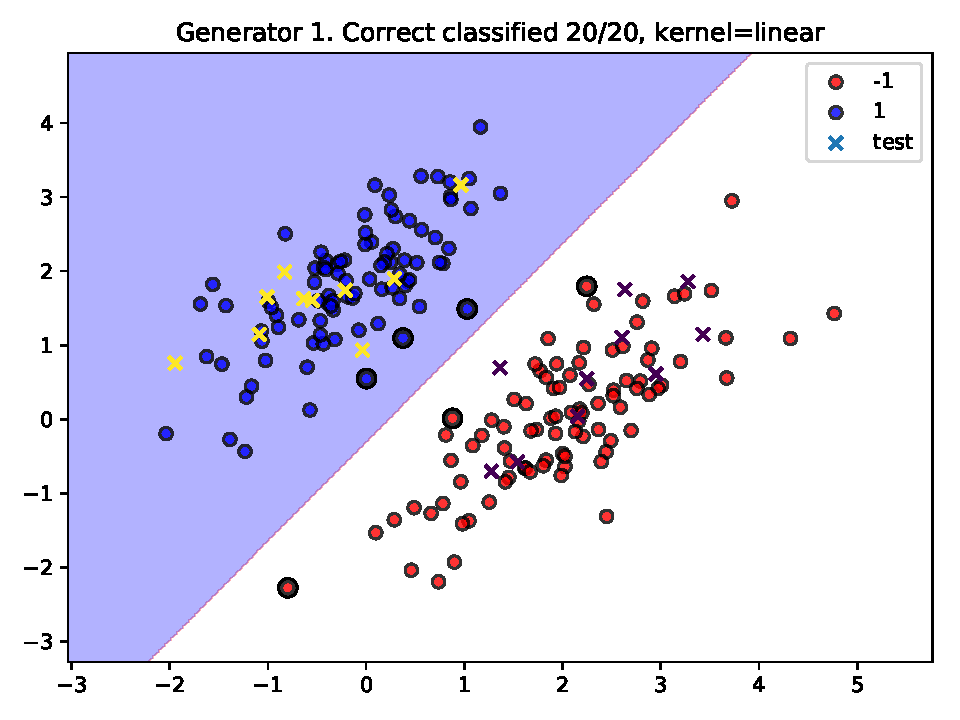
\includegraphics[width=0.7\textwidth]{ex1/1.pdf}
	\caption{Dataset of the generator 1}
	\label{fig:ex1gen1}
\end{figure}
\begin{figure}[h]
	\centering
	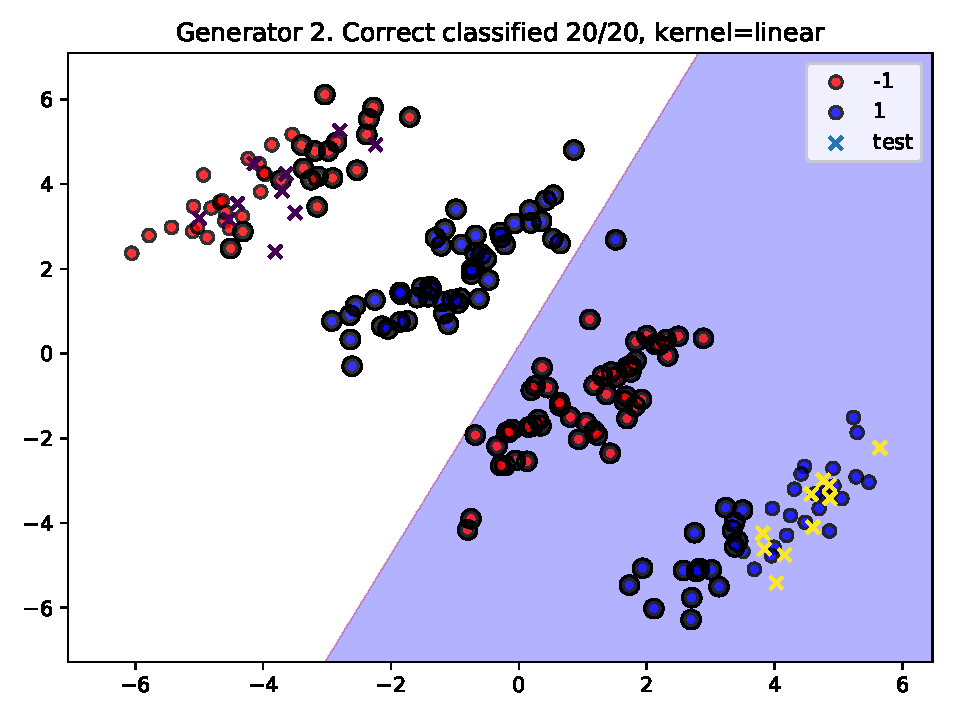
\includegraphics[width=0.7\textwidth]{ex1/2.pdf}
	\caption{Dataset of the generator 2}
	\label{fig:ex1gen2}
\end{figure}
\begin{figure}[h]
	\centering
	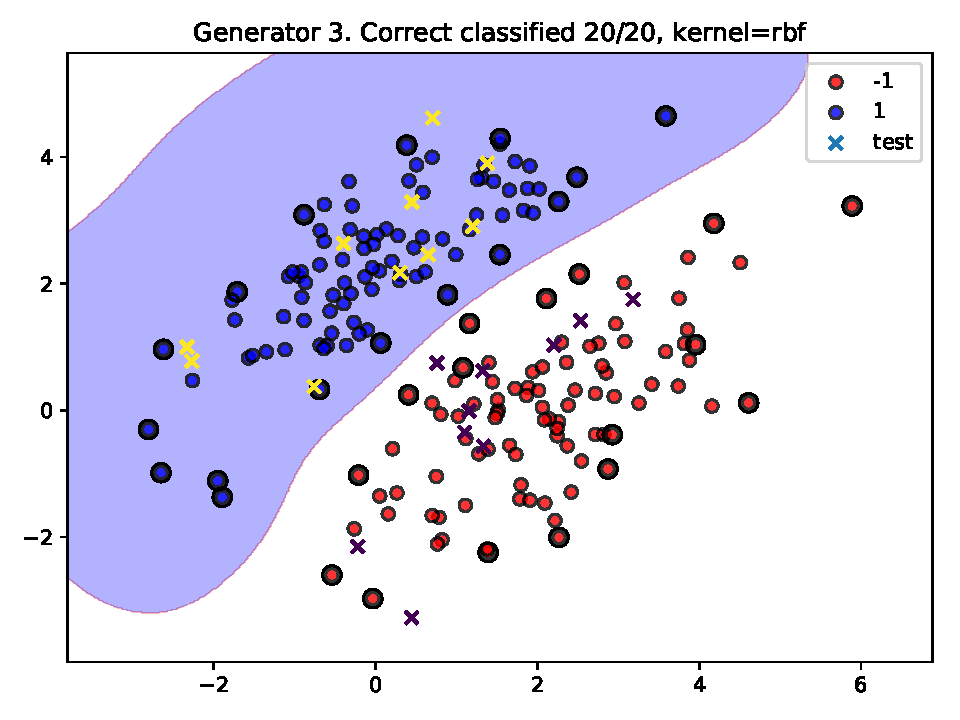
\includegraphics[width=0.7\textwidth]{ex1/3.pdf}
	\caption{Dataset of the generator 3}
	\label{fig:ex1gen3}
\end{figure}
\begin{figure}[h]
	\centering
	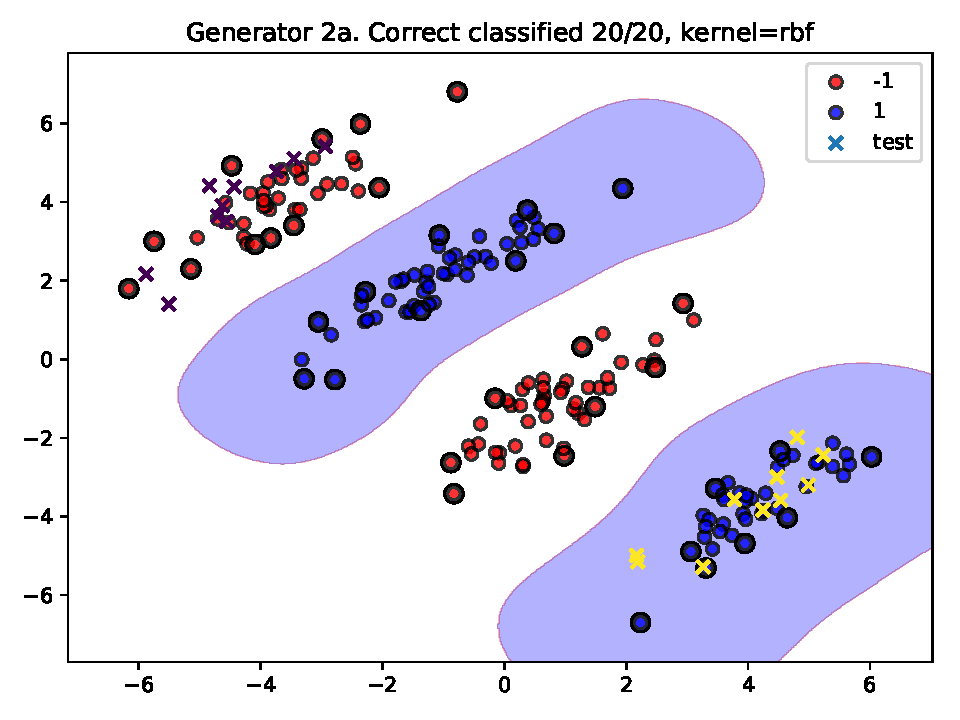
\includegraphics[width=0.7\textwidth]{ex1/2a.pdf}
	\caption{Dataset of the generator 2 using a Gaussian kernel}
	\label{fig:ex1gen2a}
\end{figure}
%

\section*{Exercise 2}

For the second exercise, we use the ex2.py file using the datasets hepatitis and satimage. 
We calculate the scores (accuracy) and time taken for each of the training and testing 
folds using different configuration for the SVM algorithm, changing the kernel types to use
(in this case the linear, radial basis function or polynomial) and the penalty “C” parameter
value (0.7, 1, 1.3). The resulting scores of each of the fold datasets from each configuration
setting are averaged and the best option with the highest score is considered the best choice.
In the Figures 5 and 6, the results of the exercise 2 execution are shown, with the
configuration combination used, the average resulting score and the execution time. The SVM
function used is the one from sklearn \footnote{http://scikit-learn.org/stable/modules/generated/sklearn.svm.SVC.html}. The classifiers where chosen according to different 
data model types. For linear model, for linear cases, the RBF and polynomial are used since 
they are the most commonly used for nonlinear SVMs \footnote{https://nlp.stanford.edu/IR-book/html/htmledition/nonlinear-svms-1.html}

\begin{lstlisting}[caption=Result of exercise 2 with hepatitis dataset]
	dataset hepatitis 	conf ('linear', 0.7) 	score 0.876 	 time 1.259e-03
	dataset hepatitis 	conf ('linear', 1) 	score 0.876 	 time 1.083e-03
	dataset hepatitis 	conf ('linear', 1.3) 	score 0.876 	 time 1.141e-03
	dataset hepatitis 	conf ('rbf', 0.7) 	score 0.836 	 time 1.333e-03
	dataset hepatitis 	conf ('rbf', 1) 	           score 0.834 	 time 1.272e-03
	dataset hepatitis 	conf ('rbf', 1.3) 	score 0.840 	 time 1.254e-03
	dataset hepatitis 	conf ('poly', 0.7) 	score 0.832 	 time 9.656e-04
	dataset hepatitis 	conf ('poly', 1) 	score 0.818 	 time 9.818e-04
	dataset hepatitis 	conf ('poly', 1.3) 	score 0.818 	 time 9.575e-04

	Best configuration ('linear', 1) with score 0.876 and time 1.083e-03	
\end{lstlisting}

\begin{lstlisting}[caption=Result of exercise 2 with satimage dataset]
	dataset satimage 	conf ('linear', 0.7) 	score 0.872 	 time 6.747e-01
	dataset satimage 	conf ('linear', 1) 	score 0.873 	 time 6.970e-01
	dataset satimage 	conf ('linear', 1.3) 	score 0.872 	 time 7.432e-01
	dataset satimage 	conf ('rbf', 0.7) 	score 0.896 	 time 1.386e+00
	dataset satimage 	conf ('rbf', 1) 	           score 0.899 	 time 1.316e+00
	dataset satimage 	conf ('rbf', 1.3) 	score 0.902 	 time 1.296e+00
	dataset satimage 	conf ('poly', 0.7) 	score 0.862 	 time 9.430e-01
	dataset satimage 	conf ('poly', 1) 	score 0.867 	 time 8.734e-01
	dataset satimage 	conf ('poly', 1.3) 	score 0.868 	 time 7.972e-01

	Best configuration ('rbf', 1.3) with score 0.902 and time 1.296e+00	
\end{lstlisting}

\section*{Analysis}

- Which is the best kernel function for a SVM classifier?
The best kernel functions depend on the type of the model, and how much we know beforehand.
If we know that the data can be separated linearly, then a linear classifier will be the
best option since it may save computational time and could prevent overfitting the data. 
In the exercise 1, for the dataset 2, we can visualize how the linear classifier doesn’t 
classify the data correctly (Figure 2) and then how the classification is made better when 
using the RBF classifier (Figure 4) so, for non-linear cases, a linear classifier may not 
have a good accuracy, so usually the RBF (Radial Basis Function or Gaussian) is more commonly 
used since it can better adapt to any type of data model \footnote{https://www.int-arch-photogramm-remote-sens-spatial-inf-sci.net/XL-2-W3/281/2014/isprsarchives-XL-2-W3-281-2014.pdf} \footnote{https://www.kdnuggets.com/2016/06/select-support-vector-machine-kernels.html}. Based on the results of the exercise, 
this statement can be reaffirmed since the best results for non-linear models where obtained 
using the RBF classifier. But overall, there is not a “best” kernel function to use for a 
SVM classifier since the results can be different for different models. 

- Did you find differences in performance among the different kernel functions used at 
the SVM algorithm?
The difference in performance can be best examined in the satimage dataset, since it is 
the dataset with the most amount of samples so the differences are more evident than in the 
other cases, but still some analysis could be established from the hepatitis dataset.

\begin{itemize}
\item For the satimage dataset:
	\begin{itemize}
		\item The combination with the best performance was the linear classifier and a C value of 0.7, this because the linear classifier requires less mathematical operations than other cases, but still has a low accuracy compared to the other combinations. 
		\item The polynomial classifier has the second best performance output but has the lowest accuracy of the three functions.
	\end{itemize}
\item For the hepatitis dataset:
	\begin{itemize}
		\item The best performing classifier was the polynomial classifier but it is also the one with the least accuracy.
		\item The linear and RBF classifiers took about the same time executing, with the difference being that the linear obtained the best accuracy results
		
	\end{itemize} 
So overall, the polynomial classifier can sometimes outperform the other classifiers, but its accuracy is not as good and the RBF classifier seems to be the one that has the least performance for these datasets.
\end{itemize}

- According to the data sets chosen, in both exercises, which combination of hyperparameters let you to improve at the maximum the accuracy of the SVM?

\section*{Execution}

To execute the code, simply run each of the .py files included (ex1.py and ex2.py) as a 
python program. Example: python ex1.py or python ex2.py

\end{document}
